%****************************************************************************************************************************************
% File: mpm-ontology.tex
%
% This file is automatically generated. Please do not edit!
%****************************************************************************************************************************************
\section{Ontology Overview}

This ontology captures the Multi-Paradigm Modeling Domain (MPM). It includes concepts for the related modeling, linguistic and formal sub domains.

Figure \ref{fig:mpm_ontology_overview} shows an overview of the MPM ontology. The details of each concept are
provided in the following subsections.

\begin{figure}[!htb]
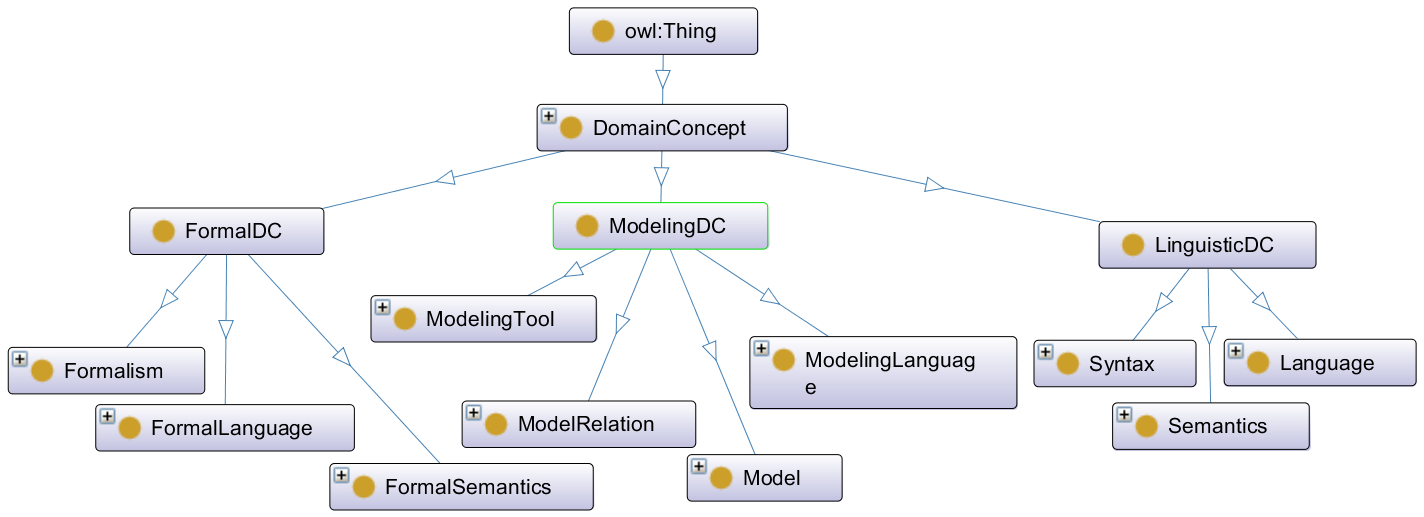
\includegraphics[width=\textwidth]{figures/mpm_ontology_overview.png}
\caption{Overview of the MPM ontology}
\label{fig:mpm_ontology_overview}
\end{figure}



\section{Domain Concepts}

This ontology of multi-paradigm modeling contains concepts divided into sub-domains as presented in the following subsections.

\subsection{ModelingDC}
\label{subsecDC:ModelingDC}

The ModelingDC subdomain organizes modeling concepts related to core modeling, multi-formalism and model management. It extends several notions introduced in a generic way by the shared ontology such as Language subclassed into ModelingLanguage and Tool subclassed into ModelingTool.

It precises the core notions of Model, ModelRelation, ModelingLanguage, AbstractSyntax, ConcreteSyntax, etc., as well as the core model management notions related to megamodeling such as Megamodel, MegamodelFragment, ModelRelation, etc.

\subsubsection{AbstractSyntax}
\label{subsubsecC:AbstractSyntax}
\didx{AbstractSyntax}

An abstract syntax is a syntax that only captures the essence of a language (its concepts and the relations between them) independently from the notation users will employ to manipulate models of the language. An abstract syntax is equivalent to the Abstract Syntax Trees (ASTs) into which code of programming languages are transformed during compilation

\textbf{Subclass of}
\begin{itemize}
	\item \textbf{Model} (see section \ref{subsubsecC:Model})
	\item \textbf{Syntax} (see section \ref{subsubsecC:Syntax})
\end{itemize}






\subsubsection{AnalysisTool}
\label{subsubsecC:AnalysisTool}
\didx{AnalysisTool}

Tools to analysis systems e.g. performance, resourceConsumption, schedulability ....

\textbf{Subclass of}
\begin{itemize}
	\item \textbf{ModelingTool} (see section \ref{subsubsecC:ModelingTool})
\end{itemize}






\subsubsection{ApplicationMegaModel}
\label{subsubsecC:ApplicationMegaModel}
\didx{ApplicationMegaModel}

A representation of the real models in the CPS development environment.

\textbf{Subclass of}
\begin{itemize}
	\item \textbf{Megamodel} (see section \ref{subsubsecC:Megamodel})
\end{itemize}






\subsubsection{ArchitectureDescriptionLanguage}
\label{subsubsecC:ArchitectureDescriptionLanguage}
\didx{ArchitectureDescriptionLanguage}

The notion of software architecture has been proposed, since the early 1990s by Perry and Wolf, as a software system representation composed of a set
of components with their interactions and their constraints. 
A software architecture is designed using an architectural language (may also be referred to as ADL (Architectural Description Language)), which is generally defined as any form of expression for use in architecture descriptions, according to the ISO/IEC/IEEE standard.

\textbf{Subclass of}
\begin{itemize}
	\item \textbf{ModelingLanguage} (see section \ref{subsubsecC:ModelingLanguage})
\end{itemize}






\subsubsection{AutomataBasedFormalism}
\label{subsubsecC:AutomataBasedFormalism}
\didx{AutomataBasedFormalism}

The class of formalisms that are based on automata

\textbf{Subclass of}
\begin{itemize}
	\item \textbf{Formalism} (see section \ref{subsubsecC:Formalism})
\end{itemize}






\subsubsection{BehavioralADL}
\label{subsubsecC:BehavioralADL}
\didx{BehavioralADL}

Behavioral Architectural Description Languages describe the behavior as a property of the components that constitute the architecture.

\textbf{Subclass of}
\begin{itemize}
	\item \textbf{ArchitectureDescriptionLanguage} (see section \ref{subsubsecC:ArchitectureDescriptionLanguage})
\end{itemize}






\subsubsection{BehavioralCharacteristic}
\label{subsubsecC:BehavioralCharacteristic}
\didx{BehavioralCharacteristic}

Behavioral characteristics of the formalism.

\textbf{Subclass of}
\begin{itemize}
	\item \textbf{FormalismCharacteristic} (see section \ref{subsubsecC:FormalismCharacteristic})
\end{itemize}






\subsubsection{CapturingOperation}
\label{subsubsecC:CapturingOperation}
\didx{CapturingOperation}

Capturing Operation

\textbf{Subclass of}
\begin{itemize}
	\item \textbf{TransformationRelation} (see section \ref{subsubsecC:TransformationRelation})
\end{itemize}






\subsubsection{CommunicationADL}
\label{subsubsecC:CommunicationADL}
\didx{CommunicationADL}

Communication Architecture Description Languages describe the architecture on the basis of the communication and coordination between the subcomponents, useful especially if the components are physically distributed processes.

\textbf{Subclass of}
\begin{itemize}
	\item \textbf{ArchitectureDescriptionLanguage} (see section \ref{subsubsecC:ArchitectureDescriptionLanguage})
\end{itemize}






\subsubsection{ConcreteModelingLanguage}
\label{subsubsecC:ConcreteModelingLanguage}
\didx{ConcreteModelingLanguage}

The notion of concrete language is defined as a language that comprises both an abstract syntax and a concrete syntax mapping function k.

\textbf{Subclass of}
\begin{itemize}
	\item \textbf{ModelingLanguage} (see section \ref{subsubsecC:ModelingLanguage})
\end{itemize}






\subsubsection{ConcreteSyntax}
\label{subsubsecC:ConcreteSyntax}
\didx{ConcreteSyntax}

A concrete syntax is the syntax users of the language manipulate to build models of the language. A modeling language may have several concrete syntaxes such as textual and graphical ones to improve its usability.

\textbf{Subclass of}
\begin{itemize}
	\item \textbf{Model} (see section \ref{subsubsecC:Model})
	\item \textbf{Syntax} (see section \ref{subsubsecC:Syntax})
\end{itemize}






\subsubsection{ConfigurationMegaModel}
\label{subsubsecC:ConfigurationMegaModel}
\didx{ConfigurationMegaModel}

Declares types for the models and relations contained in application megamodel. (language and relation types)

\textbf{Subclass of}
\begin{itemize}
	\item \textbf{Megamodel} (see section \ref{subsubsecC:Megamodel})
\end{itemize}






\subsubsection{ConformanceRelation}
\label{subsubsecC:ConformanceRelation}
\didx{ConformanceRelation}

A ConformanceRelation is a subclass of the ModelRelation to relate  a Metamodel with its conforming MicroModel(s).

\textbf{Subclass of}
\begin{itemize}
	\item \textbf{ModelRelation} (see section \ref{subsubsecC:ModelRelation})
\end{itemize}






\subsubsection{ContinuousCharacteristic}
\label{subsubsecC:ContinuousCharacteristic}
\didx{ContinuousCharacteristic}

Continuous Characteristic represents the behavioral characteristics of the formalism that are continuous in nature.

\textbf{Subclass of}
\begin{itemize}
	\item \textbf{BehavioralCharacteristic} (see section \ref{subsubsecC:BehavioralCharacteristic})
\end{itemize}






\subsubsection{DiscreteCharacteristic}
\label{subsubsecC:DiscreteCharacteristic}
\didx{DiscreteCharacteristic}

Discrete Characteristic represents the behavioral characteristics of the formalism that are discrete in nature.

\textbf{Subclass of}
\begin{itemize}
	\item \textbf{BehavioralCharacteristic} (see section \ref{subsubsecC:BehavioralCharacteristic})
\end{itemize}






\subsubsection{DomainSpecificLanguage}
\label{subsubsecC:DomainSpecificLanguage}
\didx{DomainSpecificLanguage}

The DSLs are specialized languages which capture the concepts of a specific domain.

\textbf{Subclass of}
\begin{itemize}
	\item \textbf{ModelingLanguage} (see section \ref{subsubsecC:ModelingLanguage})
\end{itemize}






\subsubsection{ExecutionTool}
\label{subsubsecC:ExecutionTool}
\didx{ExecutionTool}

Execution Tool

\textbf{Subclass of}
\begin{itemize}
	\item \textbf{ModelingTool} (see section \ref{subsubsecC:ModelingTool})
\end{itemize}






\subsubsection{FlowBasedFormalism}
\label{subsubsecC:FlowBasedFormalism}
\didx{FlowBasedFormalism}

Flow-based Formalisms

\textbf{Subclass of}
\begin{itemize}
	\item \textbf{Formalism} (see section \ref{subsubsecC:Formalism})
\end{itemize}






\subsubsection{FormalLanguage}
\label{subsubsecC:FormalLanguage}
\didx{FormalLanguage}

A modeling language is said to be formal if it is based on a well-defined semantics using mathematical foundations.

\textbf{Subclass of}
\begin{itemize}
	\item \textbf{ModelingLanguage} (see section \ref{subsubsecC:ModelingLanguage})
\end{itemize}






\subsubsection{Formalism}
\label{subsubsecC:Formalism}
\didx{Formalism}

Formalisms are mathematical objects consisting of an abstract
syntax and a formal semantics. Languages are concrete
implementations of formalisms. A language has a concrete
syntax, may deviate slightly from the formalism in the
semantics that it implements, or may implement multiple
semantics (e.g., changing the type of numerical solver in a
simulation tool may change the behavior of a model). Also, a
language may implement more than one formalisms.

\textbf{Subclass of}
\begin{itemize}
	\item \textbf{FormalismDC} (see section \ref{subsubsecC:FormalismDC})
	\item \textbf{Model} (see section \ref{subsubsecC:Model})
\end{itemize}


\textbf{References}
\begin{itemize}
	
\item \bibentry{Broman2012}
\end{itemize}




\subsubsection{FormalismCharacteristic}
\label{subsubsecC:FormalismCharacteristic}
\didx{FormalismCharacteristic}

Formalism characteristic.

\textbf{Subclass of}
\begin{itemize}
	\item \textbf{FormalismDC} (see section \ref{subsubsecC:FormalismDC})
\end{itemize}






\subsubsection{FormalismDC}
\label{subsubsecC:FormalismDC}
\didx{FormalismDC}

This class groups classes related to formalisms

\textbf{Subclass of}
\begin{itemize}
	\item \textbf{ModelingDC} (see section \ref{subsecDC:ModelingDC})
\end{itemize}






\subsubsection{GraphicalSyntax}
\label{subsubsecC:GraphicalSyntax}
\didx{GraphicalSyntax}

Graphical syntax display sentences of the language as visual elements such as boxes and arrows.
However pure graphical syntax are not common and often include textual parts.

\textbf{Subclass of}
\begin{itemize}
	\item \textbf{ConcreteSyntax} (see section \ref{subsubsecC:ConcreteSyntax})
\end{itemize}






\subsubsection{HybridAutomataBasedFormalism}
\label{subsubsecC:HybridAutomataBasedFormalism}
\didx{HybridAutomataBasedFormalism}

Hybrid Automata-based Formalisms

\textbf{Subclass of}
\begin{itemize}
	\item \textbf{AutomataBasedFormalism} (see section \ref{subsubsecC:AutomataBasedFormalism})
\end{itemize}






\subsubsection{LogicBasedFormalism}
\label{subsubsecC:LogicBasedFormalism}
\didx{LogicBasedFormalism}

Logic-based Formalisms

\textbf{Subclass of}
\begin{itemize}
	\item \textbf{Formalism} (see section \ref{subsubsecC:Formalism})
\end{itemize}






\subsubsection{Megamodel}
\label{subsubsecC:Megamodel}
\didx{Megamodel}

A model that contains models and relations between them.

\textbf{Subclass of}
\begin{itemize}
	\item \textbf{Model} (see section \ref{subsubsecC:Model})
\end{itemize}






\subsubsection{MegamodelFragment}
\label{subsubsecC:MegamodelFragment}
\didx{MegamodelFragment}

The fragment is not a complete megamodel, and can't be used alone. It can be reused to take part in another megamodel. (e.g. physical part, view of the system, self-adaptation .... etc.)

\textbf{Subclass of}
\begin{itemize}
	\item \textbf{Model} (see section \ref{subsubsecC:Model})
\end{itemize}





\todoAuthors{Do we add also application and configuration division here?}


\subsubsection{Metamodel}
\label{subsubsecC:Metamodel}
\didx{Metamodel}

A metamodel is a model of a model.

\textbf{Subclass of}
\begin{itemize}
	\item \textbf{Model} (see section \ref{subsubsecC:Model})
\end{itemize}






\subsubsection{MicroModelElement}
\label{subsubsecC:MicroModelElement}
\didx{MicroModelElement}

MicroModelElement represents an  atomic element contained by a MicroModel.

\textbf{Subclass of}
\begin{itemize}
	\item \textbf{Model} (see section \ref{subsubsecC:Model})
\end{itemize}






\subsubsection{Micromodel}
\label{subsubsecC:Micromodel}
\didx{Micromodel}

Micromodels are usual models and their model elements.

\textbf{Subclass of}
\begin{itemize}
	\item \textbf{Model} (see section \ref{subsubsecC:Model})
\end{itemize}






\subsubsection{Model}
\label{subsubsecC:Model}
\didx{Model}

A representation of real artifacts regardless of the metamodeling technical space. e.g. xml file, equations...etc.

\textbf{Subclass of}
\begin{itemize}
	\item \textbf{ModelingDC} (see section \ref{subsecDC:ModelingDC})
\end{itemize}






\subsubsection{ModelRelation}
\label{subsubsecC:ModelRelation}
\didx{ModelRelation}

A relation that connects models.

\textbf{Subclass of}
\begin{itemize}
	\item \textbf{ModelingDC} (see section \ref{subsecDC:ModelingDC})
	\item \textbf{ModelRelation} (see section \ref{subsubsecC:ModelRelation})
\end{itemize}






\subsubsection{ModelingLanguage}
\label{subsubsecC:ModelingLanguage}
\didx{ModelingLanguage}

ModelingLanguage extends the Language subclasse from the shared ontology.

\textbf{Subclass of}
\begin{itemize}
	\item \textbf{Model} (see section \ref{subsubsecC:Model})
	\item \textbf{Language} (see section \ref{subsubsecC:Language})
\end{itemize}






\subsubsection{ModelingParadigm}
\label{subsubsecC:ModelingParadigm}
\didx{ModelingParadigm}

A modeling paradigm is a set of properties characterizing the languages (including their semantics) and workflows (development
processes) employed to develop systems.

\textbf{Subclass of}
\begin{itemize}
	\item \textbf{ModelingDC} (see section \ref{subsecDC:ModelingDC})
\end{itemize}






\subsubsection{ModelingTool}
\label{subsubsecC:ModelingTool}
\didx{ModelingTool}

Tools to model the system.

\textbf{Subclass of}
\begin{itemize}
	\item \textbf{Model} (see section \ref{subsubsecC:Model})
	\item \textbf{Tool} (see section \ref{subsubsecC:Tool})
\end{itemize}






\subsubsection{PetriNetBasedFormalism}
\label{subsubsecC:PetriNetBasedFormalism}
\didx{PetriNetBasedFormalism}

Petri nets (also known as a place/transition net or P/T net) are formalisms for the description of distributed systems.

\textbf{Subclass of}
\begin{itemize}
	\item \textbf{Formalism} (see section \ref{subsubsecC:Formalism})
\end{itemize}






\subsubsection{ProgrammingLanguage}
\label{subsubsecC:ProgrammingLanguage}
\didx{ProgrammingLanguage}

The programming languages can be seen as a subset of modeling languages.

\textbf{Subclass of}
\begin{itemize}
	\item \textbf{ModelingLanguage} (see section \ref{subsubsecC:ModelingLanguage})
\end{itemize}






\subsubsection{RefinementRelation}
\label{subsubsecC:RefinementRelation}
\didx{RefinementRelation}

Example of a  transformation relation.

\textbf{Subclass of}
\begin{itemize}
	\item \textbf{TransformationRelation} (see section \ref{subsubsecC:TransformationRelation})
\end{itemize}






\subsubsection{RuntimeTool}
\label{subsubsecC:RuntimeTool}
\didx{RuntimeTool}

Runtime Tool

\textbf{Subclass of}
\begin{itemize}
	\item \textbf{ModelingTool} (see section \ref{subsubsecC:ModelingTool})
\end{itemize}






\subsubsection{SemanticDomain}
\label{subsubsecC:SemanticDomain}
\didx{SemanticDomain}

According to Wikipedia, a semantic domain is defined as a specific place that shares a set of meanings, or a language that holds it.

\textbf{Subclass of}
\begin{itemize}
	\item \textbf{Model} (see section \ref{subsubsecC:Model})
\end{itemize}






\subsubsection{SemanticMappingRelation}
\label{subsubsecC:SemanticMappingRelation}
\didx{SemanticMappingRelation}

A semantic mapping relation.

\textbf{Subclass of}
\begin{itemize}
	\item \textbf{ModelRelation} (see section \ref{subsubsecC:ModelRelation})
\end{itemize}






\subsubsection{SimulationTool}
\label{subsubsecC:SimulationTool}
\didx{SimulationTool}

Simulation Tool

\textbf{Subclass of}
\begin{itemize}
	\item \textbf{ModelingTool} (see section \ref{subsubsecC:ModelingTool})
\end{itemize}






\subsubsection{StructuralADL}
\label{subsubsecC:StructuralADL}
\didx{StructuralADL}

Structure Architectural Definition Languages have the capability of defining the topological/heirarchical structure of the components of the architecture. For example, pipe-and-filter architectures.

\textbf{Subclass of}
\begin{itemize}
	\item \textbf{ArchitectureDescriptionLanguage} (see section \ref{subsubsecC:ArchitectureDescriptionLanguage})
\end{itemize}






\subsubsection{StructuralConstraintLanguage}
\label{subsubsecC:StructuralConstraintLanguage}
\didx{StructuralConstraintLanguage}

A modeling language for expressing constraints.

\textbf{Subclass of}
\begin{itemize}
	\item \textbf{ModelingLanguage} (see section \ref{subsubsecC:ModelingLanguage})
\end{itemize}






\subsubsection{StructureCharacteristic}
\label{subsubsecC:StructureCharacteristic}
\didx{StructureCharacteristic}

Structural characteristics of the formalism

\textbf{Subclass of}
\begin{itemize}
	\item \textbf{FormalismCharacteristic} (see section \ref{subsubsecC:FormalismCharacteristic})
\end{itemize}






\subsubsection{SynchronizationRelation}
\label{subsubsecC:SynchronizationRelation}
\didx{SynchronizationRelation}

Example of a  transformation relation.

\textbf{Subclass of}
\begin{itemize}
	\item \textbf{TransformationRelation} (see section \ref{subsubsecC:TransformationRelation})
\end{itemize}






\subsubsection{SyntaxMappingRelation}
\label{subsubsecC:SyntaxMappingRelation}
\didx{SyntaxMappingRelation}

Abstract and concrete syntaxes are related via a SyntaxMappingRelation  class that associates element(s) of a concrete syntax to represent element(s) of the abstract syntax.

\textbf{Subclass of}
\begin{itemize}
	\item \textbf{ModelRelation} (see section \ref{subsubsecC:ModelRelation})
\end{itemize}






\subsubsection{TextualSyntax}
\label{subsubsecC:TextualSyntax}
\didx{TextualSyntax}

A textual syntax consists of sequences of characters taken from an alphabet and grouped into words or tokens. 
Only some sequences of words or sentences are considered valid and the set of all valid sentences is said to make up the language.

\textbf{Subclass of}
\begin{itemize}
	\item \textbf{ConcreteSyntax} (see section \ref{subsubsecC:ConcreteSyntax})
\end{itemize}






\subsubsection{TimedAutomataBasedFormalism}
\label{subsubsecC:TimedAutomataBasedFormalism}
\didx{TimedAutomataBasedFormalism}

Timed Automata-based Formalisms

\textbf{Subclass of}
\begin{itemize}
	\item \textbf{HybridAutomataBasedFormalism} (see section \ref{subsubsecC:HybridAutomataBasedFormalism})
\end{itemize}






\subsubsection{TimedCharacteristic}
\label{subsubsecC:TimedCharacteristic}
\didx{TimedCharacteristic}

Timed Characteristic  represents the behavioral characteristics of the formalism that are time-bound.

\textbf{Subclass of}
\begin{itemize}
	\item \textbf{BehavioralCharacteristic} (see section \ref{subsubsecC:BehavioralCharacteristic})
\end{itemize}






\subsubsection{TraceabilityModel}
\label{subsubsecC:TraceabilityModel}
\didx{TraceabilityModel}

After or while a transformation is being executed, the transformed models often need to be related and a set of traceability relations are created as a by-product of the transformation execution.

\textbf{Subclass of}
\begin{itemize}
	\item \textbf{Micromodel} (see section \ref{subsubsecC:Micromodel})
\end{itemize}






\subsubsection{TraceabilityRelation}
\label{subsubsecC:TraceabilityRelation}
\didx{TraceabilityRelation}

A traceability relation is a technique to provide a relationship between requirements, design, and final implementation of a system.

\textbf{Subclass of}
\begin{itemize}
	\item \textbf{ModelRelation} (see section \ref{subsubsecC:ModelRelation})
\end{itemize}






\subsubsection{TransformationLanguage}
\label{subsubsecC:TransformationLanguage}
\didx{TransformationLanguage}

A langauge to specify model transformations.

\textbf{Subclass of}
\begin{itemize}
	\item \textbf{ModelingLanguage} (see section \ref{subsubsecC:ModelingLanguage})
\end{itemize}






\subsubsection{TransformationRelation}
\label{subsubsecC:TransformationRelation}
\didx{TransformationRelation}

A Transformation Relation

\textbf{Subclass of}
\begin{itemize}
	\item \textbf{ModelRelation} (see section \ref{subsubsecC:ModelRelation})
\end{itemize}






\subsubsection{TransformationTool}
\label{subsubsecC:TransformationTool}
\didx{TransformationTool}

Transformation Tool

\textbf{Subclass of}
\begin{itemize}
	\item \textbf{ModelingTool} (see section \ref{subsubsecC:ModelingTool})
\end{itemize}






\subsubsection{UncertaintyCharacteristic}
\label{subsubsecC:UncertaintyCharacteristic}
\didx{UncertaintyCharacteristic}

Uncertainty Characteristic  represents the behavioral characteristics of the formalism that have uncertainty.

\textbf{Subclass of}
\begin{itemize}
	\item \textbf{BehavioralCharacteristic} (see section \ref{subsubsecC:BehavioralCharacteristic})
\end{itemize}






\subsubsection{VisualizationTool}
\label{subsubsecC:VisualizationTool}
\didx{VisualizationTool}

Visualization Tool

\textbf{Subclass of}
\begin{itemize}
	\item \textbf{ModelingTool} (see section \ref{subsubsecC:ModelingTool})
\end{itemize}

\section{Properties}
\label{sec:mpm:properties}


\subsection{hasAbstractSyntax}
\label{subsecP:hasAbstractSyntax}
The hasAbstractSyntax object property is a subproperty of the hasSyntax object property of the linguistic subdomain to relate the  ModelingLanguage and AbstractSyntax classes.

Subproperty of:
\begin{itemize}
	\item \textbf{hasSyntax} (see section \ref{subsecP:hasSyntax})
\end{itemize}


Domains:
\begin{itemize}
	\item \textbf{ModelingLanguage} (see section \ref{subsubsecC:ModelingLanguage})
\end{itemize}


Ranges:
\begin{itemize}
	\item \textbf{AbstractSyntax} (see section \ref{subsubsecC:AbstractSyntax})
\end{itemize}




\subsection{hasAbstractSyntaxSem}
\label{subsecP:hasAbstractSyntaxSem}
The hasAbstractSyntaxSem object property links the mapping relation to the mapped abstract syntax.

Subproperty of:
\begin{itemize}
	\item \textbf{hasConnectedModel} (see section \ref{subsecP:hasConnectedModel})
\end{itemize}


Domains:
\begin{itemize}
	\item \textbf{SemanticMappingRelation} (see section \ref{subsubsecC:SemanticMappingRelation})
\end{itemize}


Ranges:
\begin{itemize}
	\item \textbf{AbstractSyntax} (see section \ref{subsubsecC:AbstractSyntax})
\end{itemize}




\subsection{hasCharacteristic}
\label{subsecP:hasCharacteristic}
The hasCharacteristics relates a Formalism with a characteristic.

Subproperty of:
None


Domains:
\begin{itemize}
	\item \textbf{Formalism} (see section \ref{subsubsecC:Formalism})
\end{itemize}


Ranges:
\begin{itemize}
	\item \textbf{FormalismCharacteristic} (see section \ref{subsubsecC:FormalismCharacteristic})
\end{itemize}




\subsection{hasConcreteSyntax}
\label{subsecP:hasConcreteSyntax}
The hasAbstractSyntax object property is a subproperty of the hasSyntax object property of the linguistic subdomain, relating a ModelingLanguage with its  AbstractSyntax.

Subproperty of:
None


Domains:
\begin{itemize}
	\item \textbf{SyntaxMappingRelation} (see section \ref{subsubsecC:SyntaxMappingRelation})
\end{itemize}


Ranges:
\begin{itemize}
	\item \textbf{ConcreteSyntax} (see section \ref{subsubsecC:ConcreteSyntax})
\end{itemize}




\subsection{hasConformedModel}
\label{subsecP:hasConformedModel}
The hasConnectedModels object property links a  ConformanceRelation to MicroModel.

Subproperty of:
\begin{itemize}
	\item \textbf{hasConnectedModel} (see section \ref{subsecP:hasConnectedModel})
\end{itemize}


Domains:
\begin{itemize}
	\item \textbf{ConformanceRelation} (see section \ref{subsubsecC:ConformanceRelation})
\end{itemize}


Ranges:
\begin{itemize}
	\item \textbf{Micromodel} (see section \ref{subsubsecC:Micromodel})
\end{itemize}




\subsection{hasConnectedModel}
\label{subsecP:hasConnectedModel}
The model relation is used to connect an arbitrary number of models. This connects reference is defined in our ontology by the hasConnectedModels object property.

Subproperty of:
None


Domains:
\begin{itemize}
	\item \textbf{ModelRelation} (see section \ref{subsubsecC:ModelRelation})
\end{itemize}


Ranges:
\begin{itemize}
	\item \textbf{Model} (see section \ref{subsubsecC:Model})
\end{itemize}




\subsection{hasContainedMegamodelFragments}
\label{subsecP:hasContainedMegamodelFragments}
It describes the relation between megamodel and its fragments.

Subproperty of:
\begin{itemize}
	\item \textbf{hasContainedModels} (see section \ref{subsecP:hasContainedModels})
\end{itemize}


Domains:
\begin{itemize}
	\item \textbf{Megamodel} (see section \ref{subsubsecC:Megamodel})
\end{itemize}


Ranges:
\begin{itemize}
	\item \textbf{MegamodelFragment} (see section \ref{subsubsecC:MegamodelFragment})
\end{itemize}




\subsection{hasContainedModelElements}
\label{subsecP:hasContainedModelElements}
It describes the relation between micromodel and its elements.

Subproperty of:
\begin{itemize}
	\item \textbf{hasContainedModels} (see section \ref{subsecP:hasContainedModels})
\end{itemize}


Domains:
\begin{itemize}
	\item \textbf{Micromodel} (see section \ref{subsubsecC:Micromodel})
\end{itemize}


Ranges:
\begin{itemize}
	\item \textbf{MicroModelElement} (see section \ref{subsubsecC:MicroModelElement})
\end{itemize}




\subsection{hasContainedModelRelations}
\label{subsecP:hasContainedModelRelations}
A model relation also needs to be contained in a model and therefore we create the hasContainedModelRelations object property whose domain is Model and range ModelRelation.

Subproperty of:
None


Domains:
\begin{itemize}
	\item \textbf{Model} (see section \ref{subsubsecC:Model})
\end{itemize}


Ranges:
\begin{itemize}
	\item \textbf{ModelRelation} (see section \ref{subsubsecC:ModelRelation})
\end{itemize}




\subsection{hasContainedModels}
\label{subsecP:hasContainedModels}
It describes a recursive relation. e.g. MegaModelFragment hasModel xModel ...

Subproperty of:
None


Domains:
\begin{itemize}
	\item \textbf{Model} (see section \ref{subsubsecC:Model})
\end{itemize}


Ranges:
\begin{itemize}
	\item \textbf{Model} (see section \ref{subsubsecC:Model})
\end{itemize}




\subsection{hasContextRelation}
\label{subsecP:hasContextRelation}
A model relation may exist in the context of another model relation. This is expressed by  the hasContextRelation object property in the ontology. An example of such contextual relation may be a relation between to model elements that can only exist after a relation has first been created between their respective containing parent elements.

Subproperty of:
None


Domains:
\begin{itemize}
	\item \textbf{ModelRelation} (see section \ref{subsubsecC:ModelRelation})
\end{itemize}


Ranges:
\begin{itemize}
	\item \textbf{ModelRelation} (see section \ref{subsubsecC:ModelRelation})
\end{itemize}




\subsection{hasCoreLanguage}
\label{subsecP:hasCoreLanguage}
\todoAuthors{Provide ``rdfs:comment'' annotation in ontology}

Subproperty of:
None


Domains:
\begin{itemize}
	\item \textbf{ModelingLanguage} (see section \ref{subsubsecC:ModelingLanguage})
\end{itemize}


Ranges:
\begin{itemize}
	\item \textbf{ModelingLanguage} (see section \ref{subsubsecC:ModelingLanguage})
\end{itemize}




\subsection{hasInputModel}
\label{subsecP:hasInputModel}
It describes the input model for a model relation.

Subproperty of:
None


Domains:
\begin{itemize}
	\item \textbf{ModelRelation} (see section \ref{subsubsecC:ModelRelation})
\end{itemize}


Ranges:
\begin{itemize}
	\item \textbf{Model} (see section \ref{subsubsecC:Model})
\end{itemize}




\subsection{hasLanguage}
\label{subsecP:hasLanguage}
\todoAuthors{Provide ``rdfs:comment'' annotation in ontology}

Subproperty of:
None


Domains:
\begin{itemize}
	\item \textbf{Micromodel} (see section \ref{subsubsecC:Micromodel})
\end{itemize}


Ranges:
\begin{itemize}
	\item \textbf{ModelingLanguage} (see section \ref{subsubsecC:ModelingLanguage})
\end{itemize}




\subsection{hasLanguageFragment}
\label{subsecP:hasLanguageFragment}
\todoAuthors{Provide ``rdfs:comment'' annotation in ontology}

Subproperty of:
None


Domains:
\begin{itemize}
	\item \textbf{ModelingLanguage} (see section \ref{subsubsecC:ModelingLanguage})
\end{itemize}


Ranges:
None




\subsection{hasMetamodel}
\label{subsecP:hasMetamodel}
The hasMetamodel object property is a subproperty of the hasConnectedModels object property with its domain and range respectively refined to ConformanceRelation and Metamodel

Subproperty of:
\begin{itemize}
	\item \textbf{hasConnectedModel} (see section \ref{subsecP:hasConnectedModel})
\end{itemize}


Domains:
\begin{itemize}
	\item \textbf{ConformanceRelation} (see section \ref{subsubsecC:ConformanceRelation})
\end{itemize}


Ranges:
\begin{itemize}
	\item \textbf{Metamodel} (see section \ref{subsubsecC:Metamodel})
\end{itemize}




\subsection{hasOutputModel}
\label{subsecP:hasOutputModel}
It describes the output model for a model relation.

Subproperty of:
None


Domains:
\begin{itemize}
	\item \textbf{ModelRelation} (see section \ref{subsubsecC:ModelRelation})
\end{itemize}


Ranges:
\begin{itemize}
	\item \textbf{Model} (see section \ref{subsubsecC:Model})
\end{itemize}




\subsection{hasSemanticDomain}
\label{subsecP:hasSemanticDomain}
The hasSemanticDomain object properties links the mapping relation to  its semantic domain.

Subproperty of:
\begin{itemize}
	\item \textbf{hasConnectedModel} (see section \ref{subsecP:hasConnectedModel})
\end{itemize}


Domains:
\begin{itemize}
	\item \textbf{SemanticMappingRelation} (see section \ref{subsubsecC:SemanticMappingRelation})
\end{itemize}


Ranges:
\begin{itemize}
	\item \textbf{SemanticDomain} (see section \ref{subsubsecC:SemanticDomain})
\end{itemize}




\subsection{hasSpecification}
\label{subsecP:hasSpecification}
a TransformationRelation class is a subclass of the ModelRelation class with an object property hasSpecification
to relate the transformation relation to its specification.

Subproperty of:
None


Domains:
\begin{itemize}
	\item \textbf{TransformationRelation} (see section \ref{subsubsecC:TransformationRelation})
\end{itemize}


Ranges:
\begin{itemize}
	\item \textbf{Micromodel} (see section \ref{subsubsecC:Micromodel})
\end{itemize}




\subsection{hasSyntaxMapping}
\label{subsecP:hasSyntaxMapping}
The hasSyntaxMapping relates  a ConcreteModelingLanguage to its SyntaxMappingRelation.

Subproperty of:
None


Domains:
\begin{itemize}
	\item \textbf{ConcreteModelingLanguage} (see section \ref{subsubsecC:ConcreteModelingLanguage})
\end{itemize}


Ranges:
\begin{itemize}
	\item \textbf{SyntaxMappingRelation} (see section \ref{subsubsecC:SyntaxMappingRelation})
\end{itemize}




\subsection{hasTool}
\label{subsecP:hasTool}
This object property relates a modelling language to the tool(s) that implement it,

Subproperty of:
None


Domains:
\begin{itemize}
	\item \textbf{ModelingLanguage} (see section \ref{subsubsecC:ModelingLanguage})
\end{itemize}


Ranges:
\begin{itemize}
	\item \textbf{ModelingTool} (see section \ref{subsubsecC:ModelingTool})
\end{itemize}




\subsection{hasTraceabilityRelation}
\label{subsecP:hasTraceabilityRelation}
The hasContainedModelRelations is refined into the hasTraceabilityRelation with the domain and the range respectively refined into TraceabilityModel and TraceabilityRelation.

Subproperty of:
\begin{itemize}
	\item \textbf{hasContainedModelRelations} (see section \ref{subsecP:hasContainedModelRelations})
\end{itemize}


Domains:
\begin{itemize}
	\item \textbf{TraceabilityModel} (see section \ref{subsubsecC:TraceabilityModel})
\end{itemize}


Ranges:
\begin{itemize}
	\item \textbf{TraceabilityRelation} (see section \ref{subsubsecC:TraceabilityRelation})
\end{itemize}




\subsection{hasTranformationSpecification}
\label{subsecP:hasTranformationSpecification}
The hasTranformationSpecifications object property relates an activity performer resource to the transformation relations it executes.

Subproperty of:
None


Domains:
\begin{itemize}
	\item \textbf{ActivityPerformer} (see section \ref{subsubsecC:ActivityPerformer})
\end{itemize}


Ranges:
\begin{itemize}
	\item \textbf{TransformationRelation} (see section \ref{subsubsecC:TransformationRelation})
\end{itemize}




\subsection{hasUsedModels}
\label{subsecP:hasUsedModels}
This propoerty relates the MegaModel Fragment to the MicroModel(s) it incorporates.

Subproperty of:
None


Domains:
\begin{itemize}
	\item \textbf{MegamodelFragment} (see section \ref{subsubsecC:MegamodelFragment})
\end{itemize}


Ranges:
\begin{itemize}
	\item \textbf{Micromodel} (see section \ref{subsubsecC:Micromodel})
\end{itemize}




\subsection{isBasedOn}
\label{subsecP:isBasedOn}
The relation defines the formalism for a formal language. It is an inverse of hasLanguage.

Subproperty of:
None


Domains:
\begin{itemize}
	\item \textbf{ModelingLanguage} (see section \ref{subsubsecC:ModelingLanguage})
\end{itemize}


Ranges:
\begin{itemize}
	\item \textbf{Formalism} (see section \ref{subsubsecC:Formalism})
\end{itemize}




\subsection{isEnvironmentFor}
\label{subsecP:isEnvironmentFor}
This relation is used to relate a modelling tool to its extension(s). The original modelling tool serves as an environment for the development and operation of the tool extension.

Subproperty of:
None


Domains:
\begin{itemize}
	\item \textbf{ModelingTool} (see section \ref{subsubsecC:ModelingTool})
\end{itemize}


Ranges:
None




\subsection{isImplementedBy}
\label{subsecP:isImplementedBy}
This property relates a modeling language to the formalism(s) it implements.

Subproperty of:
None


Domains:
\begin{itemize}
	\item \textbf{Formalism} (see section \ref{subsubsecC:Formalism})
\end{itemize}


Ranges:
\begin{itemize}
	\item \textbf{ModelingLanguage} (see section \ref{subsubsecC:ModelingLanguage})
\end{itemize}




\subsection{isToolExtensionFor}
\label{subsecP:isToolExtensionFor}
This property is the inverse of the isEnvironmentFor object property which relates a modelling tool and its extension(s).

Subproperty of:
None


Domains:
None


Ranges:
\begin{itemize}
	\item \textbf{ModelingTool} (see section \ref{subsubsecC:ModelingTool})
\end{itemize}




\subsection{isToolFor}
\label{subsecP:isToolFor}
This property is the inverse of hasTool object property.

Subproperty of:
None


Domains:
\begin{itemize}
	\item \textbf{ModelingTool} (see section \ref{subsubsecC:ModelingTool})
\end{itemize}


Ranges:
\begin{itemize}
	\item \textbf{ModelingLanguage} (see section \ref{subsubsecC:ModelingLanguage})
\end{itemize}




